\documentclass[sigconf,nonacm]{acmart}
% "nonacm" removes the ACM copyright/conference boilerplate but keeps the sigconf layout.
\usepackage{tikz}
\usetikzlibrary{arrows.meta}

% Red reminders. Search the file for "TODO" before submitting; remove every one.
\newcommand{\todo}[1]{{\color{red}[TODO: #1]}}

\begin{document}

\title{Passive Engagement Detection While Reading E-books\\ from Video and Interaction Signals}

\author{Alexander Santa Cruz - 1854789}
\affiliation{%
  \institution{Sapienza University of Rome}
  \city{Rome}
  \country{Italy}}

\begin{abstract}
Recommender systems for e-books rely on coarse signals such as ratings and which books are finished, which say little about
whether a reader was engaged while reading. We present a passive, browser-based prototype that estimates engagement
during a reading session without asking the reader anything. From the webcam it extracts the blink rate, long eye closures
and head movement using MediaPipe face landmarks; from the e-book reader it extracts the time on each page, to be converted into a reading rate, and the number of
times the reader goes back a page. Each measure votes, and a weighted decision-level vote gives an engaged or not engaged
verdict for the session, from which a book-level ratio of engaged sessions follows. All processing runs locally in the
browser. A calibration on a single subject shows that the thresholds separate eyes open, reading and eyes closed, and
still from moving, while a short pilot of skimming suggests that page time alone cannot reveal inattentive reading. The prototype
is implemented as a single web page, but it has not been validated on other readers or against self-reported engagement.
\end{abstract}

\maketitle

%--------------------------------------------------------------------
\section{Introduction}
Digital book platforms rely on recommendation systems to suggest what a reader should read next. These systems
combine explicit data, such as ratings and reviews, with implicit data, such as the user's behavior and choices~\cite{devika2024book}.
In practice this means coarse signals: which books a user opens, how many pages they read, whether they finished a book,
and the genres, authors and narrative styles they explore.

These signals are weak evidence of enjoyment. Explicit ratings are sparse, because users rate only a small fraction of the
available books~\cite{devika2024book}, and many readers never rate or review what they read. Finishing or
abandoning a book does not say why: a book may be finished out of duty, or put aside because of a busy period in the
reader's life and not because it was disliked. Asking readers to report their experience explicitly would
interrupt the reading and place the effort on the user.

We propose to complement existing recommenders with a measure of \emph{engagement during the reading session},
collected passively and without any input from the reader. Reading an e-book on a screen is a natural setting for this:
the device that displays the text can also observe how the reader behaves. Our prototype combines two sources of
evidence. From the webcam, it extracts blink rate, long eye closures and head movement. From the reading interface,
it extracts the time spent on each page and the number of times the reader goes back to the previous page. These cues
are largely involuntary or unreflective, so they are less likely to be shaped by the story a reader tells themselves
about a book. Knowing whether a session was engaging could then be used to weight a book's influence on future
recommendations, and it would also help readers who do not wish to explore or rate books themselves.
This use for recommendation is the motivation of the work; we do not evaluate it here.

The contributions of this paper are:
\begin{itemize}
  \item a modular, browser-based prototype that runs entirely on the user's device, with a webcam module and an
        e-book reader module;
  \item a set of video and interaction features, and a hand-specified fusion rule that turns them into an
        engaged / not engaged verdict for each reading session;
  \item a book-level metric, the ratio of engaged sessions to the total number of sessions needed to finish the book.
\end{itemize}

The rest of the paper is organized as follows. Section~\ref{sec:related} reviews related work, Section~\ref{sec:design}
describes the system architecture, Section~\ref{sec:features} the extracted features, and Section~\ref{sec:fusion} the
fusion rule and the session and book logic. Section~\ref{sec:eval} reports a preliminary calibration, and
Sections~\ref{sec:discussion} and~\ref{sec:conclusion} discuss limitations and conclude.

%--------------------------------------------------------------------
\section{Related Work}\label{sec:related}
Our work touches four areas: recommendation from implicit feedback, engagement detection from facial cues, the signals
we reuse (eye closure and reading behavior), and the browser tooling.

\paragraph{Implicit feedback in book recommendation.}
Devika and Milton~\cite{devika2024book} survey book recommender systems and describe how they combine explicit data
(ratings and reviews) with implicit data (the user's behavior and choices). They list data sparsity and the cold-start
problem among the main challenges. The implicit data in this literature are mostly interaction logs, such as which
books are opened or finished. The signal we study is a different kind of implicit feedback: it is collected
\emph{during} reading and describes how the reader behaved, not only what the reader chose.

\paragraph{Engagement detection from facial cues.}
Whitehill et al.~\cite{whitehill2014faces} trained detectors of student engagement from facial expressions and found
that the automatic judgments correlate with test performance, with accuracy close to that of human observers. Gupta et
al.~\cite{gupta2023multimodal} combine facial emotion, eye-blink count and head movement to estimate engagement in
e-learning, using simple per-modality rules whose outputs are combined into an engagement index. We take over the
rule-based, per-modality structure but differ in three ways: the context is reading a book and not watching a lesson;
the system is passive and fully local, so no video leaves the device; and it adds interaction signals from the reader
(time on page, going back) which a video lesson does not provide. We also leave out the emotion model in this prototype.

\paragraph{Eye closure and reading behavior.}
The eye aspect ratio (EAR) of Soukupov\'a and \v{C}ech~\cite{soukupova2016blink} turns six eye landmarks into one
openness value, and blinks are found by thresholding it (their baseline uses 0.2). PERCLOS, the proportion of time the
eyes are closed, is used in drowsiness detection~\cite{chang2022perclos}. These thresholds were chosen for other tasks
and conditions, and they are not directly transferable to reading, where the eyelids are lowered by looking down at the
text; we therefore measure EAR on the reading posture itself (Section~\ref{sec:features}). On the behavior side, eye
movements in reading are well studied~\cite{rayner1998eye} and silent reading speed has been summarized in a
meta-analysis~\cite{brysbaert2019words}, which we use as a reference for typical reading rate.

\paragraph{Tooling and multimodal design.}
MediaPipe~\cite{lugaresi2019mediapipe} provides face landmarks that run in the browser, which makes a fully local
prototype possible. From the multimodal interaction literature, we use the view that modalities in one system
should complement each other~\cite{reeves2004guidelines}: the video describes the body of the reader and the
interaction log describes what the reader does with the book, so one can compensate for what the other cannot see.

%--------------------------------------------------------------------
\section{System Design}\label{sec:design}
Figure~\ref{fig:overview} shows the architecture. The system has two input streams: the webcam video and the reader's
interactions with the e-book, namely the page turns and their direction. Both streams enter an Engagement Tracker,
which routes them to the analysis modules. The video is passed to MediaPipe, which returns facial landmarks for every
frame. The landmarks around the eyes (inner and outer corners, upper and lower eyelids) are used to compute the eye
aspect ratio (EAR) and are sent to the Blink Detector, and the nose landmark is sent to the Head Tracker. In parallel,
the interaction events are passed to the Touch Interaction Tracker. The outputs of the analysis modules are combined by
the Fusion Model, which produces an engaged / not engaged decision for the session that is written to a log.

\begin{figure}[t]
  \centering
  \resizebox{\columnwidth}{!}{%
  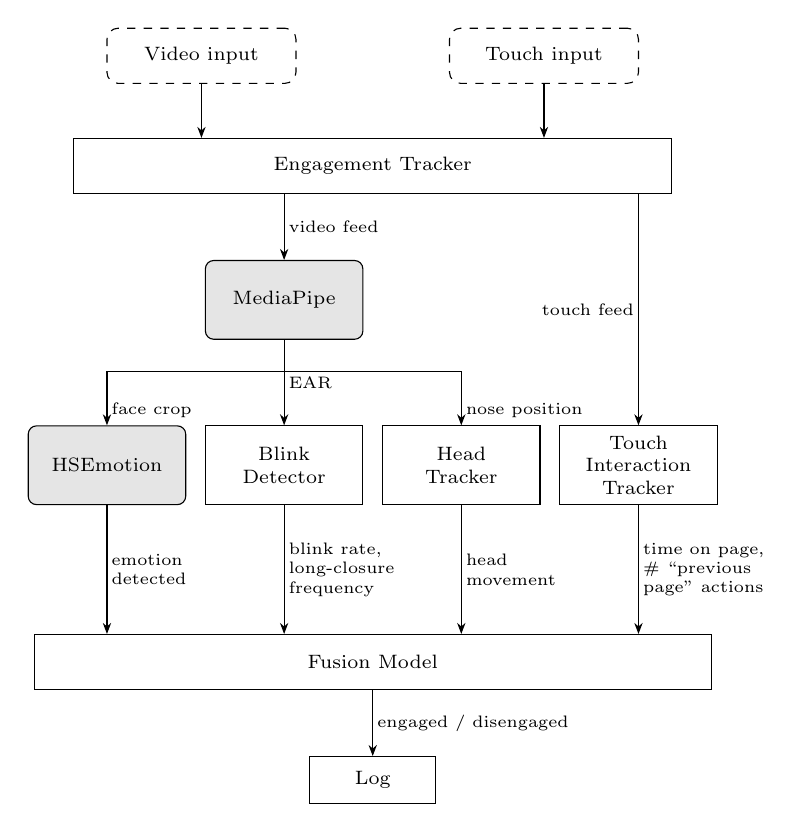
\begin{tikzpicture}[
      font=\scriptsize,
      >={Stealth[length=4pt]},
      inp/.style={draw, dashed, rounded corners=4pt, minimum width=2.4cm,
                  minimum height=0.7cm, align=center},
      mod/.style={draw, minimum width=2.0cm, minimum height=1.0cm, align=center},
      ext/.style={draw, fill=black!10, rounded corners=3pt, minimum width=2.0cm,
                  minimum height=1.0cm, align=center},
      lab/.style={font=\fontsize{6}{7}\selectfont, align=left, inner sep=1.5pt}
    ]

    % Inputs and orchestrator
    \node[inp] (video) at (2.2,0)   {Video input};
    \node[inp] (touch) at (6.55,0)  {Touch input};
    \node[mod, minimum width=7.6cm, minimum height=0.7cm] (trk) at (4.375,-1.4)
          {Engagement Tracker};

    \draw[->] (video.south) -- (video.south |- trk.north);
    \draw[->] (touch.south) -- (touch.south |- trk.north);

    % Face pipeline
    \node[ext] (mp)    at (3.25,-3.1) {MediaPipe};
    \node[ext] (emo)   at (1.0,-5.2)  {HSEmotion};
    \node[mod] (blink) at (3.25,-5.2) {Blink\\Detector};
    \node[mod] (head)  at (5.5,-5.2)  {Head\\Tracker};

    % Touch pipeline
    \node[mod] (ttrk) at (7.75,-5.2) {Touch\\Interaction\\Tracker};

    \draw[->] (trk.south -| mp.north) -- (mp.north)
          node[lab, midway, right] {video feed};
    \draw[->] (trk.south -| ttrk.north) -- (ttrk.north)
          node[lab, midway, left] {touch feed};

    \draw[->] (mp.south) -- ++(0,-0.4) -| (emo.north)
          node[lab, pos=0.86, right] {face crop};
    \draw[->] (mp.south) -- (blink.north)
          node[lab, midway, right] {EAR};
    \draw[->] (mp.south) -- ++(0,-0.4) -| (head.north)
          node[lab, pos=0.86, right] {nose position};

    % Fusion and output
    \node[mod, minimum width=8.6cm, minimum height=0.7cm] (fus) at (4.375,-7.7)
          {Fusion Model};

    \draw[->] (emo.south)   -- (emo.south |- fus.north)
          node[lab, midway, right] {emotion\\detected};
    \draw[->] (blink.south) -- (blink.south |- fus.north)
          node[lab, midway, right] {blink rate,\\long-closure\\frequency};
    \draw[->] (head.south)  -- (head.south |- fus.north)
          node[lab, midway, right] {head\\movement};
    \draw[->] (ttrk.south)  -- (ttrk.south |- fus.north)
          node[lab, midway, right] {time on page,\\\# ``previous\\page'' actions};

    \node[mod, minimum width=1.6cm, minimum height=0.6cm] (log) at (4.375,-9.2) {Log};
    \draw[->] (fus.south) -- (log.north)
          node[lab, midway, right] {engaged / disengaged};
  \end{tikzpicture}%
  }
  \caption{Overview of the proposed engagement detection system. Dashed boxes
  are inputs and shaded boxes are pretrained external components (HSEmotion is planned, not implemented).
  EAR is the eye aspect ratio. The outputs of the analysis modules are combined by a
  decision-level fusion model, and the resulting engaged/disengaged decision is
  logged.}
  \Description{Block diagram. Video and touch inputs enter the Engagement
  Tracker. Video goes to MediaPipe, which feeds HSEmotion, a blink detector and
  a head tracker. Touch goes to a touch interaction tracker. The four modules
  feed a fusion model, which outputs an engaged or disengaged decision to a log.}
  \label{fig:overview}
\end{figure}

\paragraph{Modules.}
The \emph{Blink Detector} takes the EAR of each frame and outputs the number of blinks in the last 60 seconds,
sampled every 10 seconds, and the number of long eye closures.
The \emph{Head Tracker} takes the nose landmark and outputs the head movement, that is, how fast the nose moves in the
image over a window of 10 seconds.
The \emph{Touch Interaction Tracker} records, for every page, the seconds spent on it, the number of words on it and the
direction of the page turn, and outputs, for the session, the number of backtracks (``previous page'' presses) and the
average reading rate.
The \emph{Fusion Model} averages the measures over the session, turns each of them into a vote and combines the votes
(Section~\ref{sec:fusion}).

\paragraph{Design choices.}
The design follows four choices.
(i)~\emph{Passive}: the reader gives no input. The camera preview is hidden, because seeing one's own face would distract
from reading; an optional button shows only the measured values (blink rate, long closures, head movement).
(ii)~\emph{Local}: all processing runs in the browser and no video leaves the device.
(iii)~\emph{Modular}: each signal has its own module, so signals can be added or replaced independently; for example,
the emotion module (HSEmotion) is planned as future work.
(iv)~\emph{Simple and rule-based}: the system uses thresholds and a weighted vote and not a learned model, because no
labelled data of reading sessions is available and the rules are easy to inspect, as in the rule-based use of
thresholds in Gupta et al.~\cite{gupta2023multimodal}.
The prototype is a single static web page with no back end; it only needs to be served by a local static web server and runs in a modern browser.

\paragraph{Implementation and status.}
The system is written in JavaScript and uses the MediaPipe Face Landmarker for the landmarks and epub.js for the
e-book reader. Everything runs in one page. The webcam pipeline (blinks, long closures, head movement) runs in the background with the
camera preview hidden. The reader counts the words displayed on each page by taking the text between the start and the end
position that epub.js reports for the page, and records the time spent on it and the direction of the turn. The fusion
model is evaluated when the reader presses the \emph{End Session} button, which shows the measures, the votes and the verdict, and
stores the verdict in the browser so that the book-level ratio can be computed when the last page is reached.
If the camera is not available, the reader still works and the verdict uses only the reading signals; in general, a
module without data is left out and the weights of the others are renormalized.
Section~\ref{sec:eval} states which parts were tested. The code is available at \texttt{github.com/santaCruz1854789/Reading-Engagment}.

%--------------------------------------------------------------------
\section{Feature Extraction}\label{sec:features}
\subsection{Blink and eye-closure features}
The eye aspect ratio (EAR) of each eye is the vertical distance between the upper and lower eyelid landmarks divided by the
horizontal distance between the eye corners; the two eyes are averaged. We use the 3D variant, which computes the distances from the three-dimensional landmark coordinates returned by MediaPipe, so that the value changes less when the head turns or tilts than with image-plane distances alone.\footnote{Landmark indices: left eye 386/374 (eyelids) and 362/263 (corners), right eye 159/145 and 133/33.}
A closure starts when EAR $\le 0.21$ and ends when EAR $> 0.26$ (hysteresis, to avoid flicker). A closure of at most
700\,ms is a blink; one of at least 3\,s is a long closure. Blinks per minute are computed on a sliding 60\,s window
and sampled every 10\,s; while the first minute is not yet complete, the count is scaled to a rate per minute, and no sample is taken during the first 10\,s or while no face is found.
The thresholds come from the author's measurements (Table~\ref{tab:ear}): reading lowers the eyelids, so EAR while reading (at least 0.41) is lower than with the eyes open, but still well above EAR with the eyes closed (at most 0.10). A closing threshold of 0.21 and a reopening threshold of 0.26 lie in the gap between the two. The 700\,ms limit separates blinks from longer closures. During testing, relaxed blinks, which are slower and shallower than deliberate ones, were missed with stricter thresholds (0.18 and 0.31 initially), which is why the values were relaxed.

\begin{table}[t]
  \caption{EAR (3D variant, both eyes averaged) measured on the author (single subject); $n$ is the number of samples.}
  \label{tab:ear}
  \begin{tabular}{lccc}
    \toprule
    Condition & Mean & Range & $n$ \\
    \midrule
    Eyes open, looking at screen & 0.51 & 0.40--0.55 & 11 \\
    Reading & 0.44 & 0.41--0.45 & 14 \\
    Eyes closed & 0.09 & 0.07--0.10 & 10 \\
    \bottomrule
  \end{tabular}
\end{table}

A known limitation is that very quick blinks may not reach the closing threshold at webcam frame rates and are then missed.

\subsection{Head movement}
The nose-tip landmark is tracked over a sliding 10\,s window. Head movement is the path length travelled by the nose
(in normalized image coordinates) divided by the time spanned by the window, multiplied by 1000
(units: $10^{-3}$ frame widths per second). The window is cleared when the face is lost.
Two limitations follow from this choice. A single point cannot tell turning the head from moving the whole upper body,
and the value depends on the distance to the camera, because the same movement covers a larger part of the image when the
reader sits closer.

\subsection{Interaction features}
For every page, the system records the seconds spent on it and the direction of the page turn that left it; per session it
counts the backtracks (``previous page'' presses). Pages differ in the amount of text, and so do books and screen sizes,
so the time on a page is divided by the number of words displayed on it. This gives a reading rate in words per minute (WPM)
that can be compared across books. A rate far above the typical rate of silent reading, which is about 240 WPM for adults
(238 WPM for non-fiction and 260 WPM for fiction in the meta-analysis of Brysbaert~\cite{brysbaert2019words}; we use 240),
suggests skimming, and a rate far below it may indicate that attention is elsewhere.
The session reading rate is the total number of words divided by the total time over the pages left during the session, so
that short pages such as a title page count little. Counting only the first visit to each page, so that re-reading after a
backtrack does not distort the rate, is a possible refinement.

%--------------------------------------------------------------------
\section{Fusion and Session Logic}\label{sec:fusion}
The Fusion Model works at decision level: each module turns its measure into a vote (engaged or not engaged), and the
votes are combined by a weighted vote. Following the rule-based approach of Gupta et al.~\cite{gupta2023multimodal},
who combine simple per-modality rules, we use fixed thresholds and no learned parameters.

\paragraph{Session measures.}
At the end of a session (End Session button or closing the application) the system computes four measures:
the average blink rate (blinks per minute) together with the average number of long closures per window;
the average head movement; the average reading rate (words per minute); and the backtrack ratio (``previous page'' presses divided by
all page turns, forward and backward). Occasional going back is normal, for example to re-read a sentence, but frequent going back suggests that the reader loses the thread or is searching for something instead of reading on. We therefore vote engaged if at most 20\% of the page turns are backward; this cutoff is a design assumption, chosen without data.

\begin{table}[t]
  \caption{Rules that turn each measure into a vote. A vote is 1 if the session looks engaged. All values are hand-set
  starting points, not validated on labelled data.}
  \label{tab:thresholds}
  \begin{tabular}{lll}
    \toprule
    Module & Vote = 1 (engaged) if & Basis \\
    \midrule
    Eyes & blinks/min $\le 15$ and long closures $\le 3$ & \cite{gupta2023multimodal} \\
    Head & movement $< 40$ & own pilot, Table~\ref{tab:head} \\
    Reading rate & $120 \le$ WPM $\le 480$ & hand-set: 0.5--2$\times$ the typical $\approx$240 WPM \\
    Backtracks & ratio $\le 0.2$ & design assumption \\
    \bottomrule
  \end{tabular}
\end{table}

\paragraph{Session verdict.}
With votes $v_i \in \{0,1\}$ and weights $w_i$, the score is $S = \sum_i w_i v_i$ and the session is labelled
\emph{engaged} if $S \ge 0.5$. We use equal weights $w_i = 1/4$, since we have no evidence to prefer one signal over
another.

\paragraph{Illustrative example.}
Suppose that, in a session, the average blink rate is 12 per minute with 1 long closure per window, the head movement is 9,
the reading rate is 200\,WPM and 10\% of the page turns are backward. All four rules of Table~\ref{tab:thresholds} give
a vote of 1, so $S = 4 \times 0.25 = 1$ and the session is labelled engaged. If the same reader skims at 600\,WPM and
goes back on 30\% of the turns, the reading-rate and backtrack votes become 0 and $S = 0.5$, which is still
labelled engaged because the rule is $S \ge 0.5$. With a further high blink rate, $S = 0.25$ and the session is labelled not engaged.
These numbers are illustrative, not measurements.

\paragraph{Book-level metric.}
The book-level engagement is the number of engaged sessions divided by the total number of sessions needed to finish
the book.

The blink and long-closure limits (15 and 3) are taken from Gupta et al.~\cite{gupta2023multimodal}, who count blinks and
long closures per minute and designed their rules for students watching e-learning video, not for reading. They detect a
closure with a threshold of 0.20 and call a closure long when it lasts more than 10\,s; we use 3\,s, because a
closure of 10\,s is already unlikely in a reader who is awake. Since reading is known to lower the blink rate, these values
should be seen as a starting point, and not as validated limits for reading.

%--------------------------------------------------------------------
\section{Evaluation}\label{sec:eval}
This section reports a calibration and a pilot check on a single subject, the author. It is not a user study: there are
no participants, no labelled engagement data and no accuracy figures. Its purpose is to justify the thresholds of
Section~\ref{sec:fusion} and to show what the signals can and cannot separate.

\paragraph{Eye aspect ratio.} Table~\ref{tab:ear} shows the EAR of the author in three conditions. Reading and eyes-open
EAR overlap little with the eyes-closed EAR, which makes a threshold between them possible, and the reading values lie
below the eyes-open values because the eyelids are lowered when looking at text.


\paragraph{Head movement.} Table~\ref{tab:head} shows that moving the head gives values about 30 times larger than sitting still or reading
(roughly 230--290 against 3--9). A threshold anywhere between them separates the cases; we use 40, the geometric mean of the
largest still/reading value (8.49) and the smallest moving value (229.05) rounded to a simple number. With so few
measurements from one person under one lighting condition and camera distance, this shows that the measure
reacts to movement but says nothing about its accuracy for other readers.

\begin{table}[t]
  \caption{Head movement (units $10^{-3}$ frame widths per second), single subject, 10\,s windows.}
  \label{tab:head}
  \begin{tabular}{lc}
    \toprule
    Condition & Value \\
    \midrule
    Sitting still & 3.47, 8.30 \\
    Reading posture & 8.49 \\
    Moving the head & 229.05, 291.52 \\
    \bottomrule
  \end{tabular}
\end{table}

\paragraph{Reading pilot.} In a short pilot, the author read four consecutive pages of a text that he found boring, looking
at every word without taking in the content. The times on the four pages were 34.43, 41.90, 30.18 and 45.12\,s
(mean 37.9\,s). Seconds per page alone cannot tell this skimming-like reading from attentive reading, and it also
depends on how much text is on each page, which motivates the reading rate in WPM.


\paragraph{Implementation check.} The merged page was run in a browser on the e-book \emph{Romeo and Juliet}. For a page that
we counted by eye (17 words) the word count of the page was the same. In a test in which pages were turned every few
seconds, the reading rate was far above the 480 WPM limit and the reading vote was 0, and the only backward turn gave a backtrack
ratio below 0.2 and a vote of 1, so the session was labelled engaged with a score of 0.5 from the two reading votes
(the camera was blocked in the test browser, so the video modules had no data). The fusion rule was also checked on two
constructed sets of measures: one with all four votes at 1 except the backtrack ratio (score 0.75, engaged) and one with
all votes at 0 (score 0, not engaged). We did not test the video measures on the merged page with a live face; they use the
same code as the standalone webcam page that was calibrated above. Finally, detecting the last page of the book, which
triggers the book-level ratio, was not confirmed in these tests. These checks show that the pipeline runs, not that its verdicts are correct.

%--------------------------------------------------------------------
\section{Discussion and Limitations}\label{sec:discussion}
\paragraph{What the signals can and cannot tell.} The system measures attentive reading behavior; it does not measure
comprehension or enjoyment. In our pilot (Section~\ref{sec:eval}) a session of skimming looked like normal reading
in terms of page time. No single cue is enough, which is why the system combines several, but a reader who looks
at the text, blinks normally and keeps still while not taking in the content would still be labelled as engaged.

\paragraph{Limitations.}
\begin{itemize}
  \item \emph{Single subject.} All measurements come from the author, so the thresholds are not validated across readers,
        faces, glasses, lighting or camera distance.
  \item \emph{No ground truth.} Engagement is inferred by rules, and there are no labelled reading sessions or
        self-reported engagement to compare with, so we cannot report accuracy.
  \item \emph{Hand-set thresholds.} The reading-rate range and the backtrack limit are design assumptions; the blink and
        long-closure limits were developed for e-learning video and not for reading.
  \item \emph{Webcam frame rate.} A blink lasts a fraction of a second, so a low frame rate can miss quick blinks.
  \item \emph{One landmark for the head.} The nose cannot separate turning from translating, and the value depends on the
        distance to the camera.
  \item \emph{Partly tested.} The reader, the word count and the fusion were tested in a browser, but the merged page was not
        tested with a live face (see Section~\ref{sec:eval}), and the word count was checked on one book.
\end{itemize}

\paragraph{Privacy.}
All processing happens in the browser and the video is not stored or sent. The camera preview is hidden from the
reader, so a deployed version would have to tell the reader clearly that the camera is used and let them switch it off.

\paragraph{Future work.}
The next steps are to test the merged page end to end with a live face, to add the emotion module
planned in the architecture, and to calibrate the thresholds for each reader. The most important step is a user study in
which readers rate their own engagement, which would allow an ablation of the features and a comparison of the fusion rule
with the individual signals.

%--------------------------------------------------------------------
\section{Conclusion}\label{sec:conclusion}
We presented a browser-based prototype that judges whether a reading session was engaging without asking the reader
anything. It extracts blinks, long eye closures and head movement from the webcam, and the time on each page and the
backtracks from the reader, and it combines them by a weighted vote into a verdict for each session, and into the ratio of
engaged sessions for a book. The calibration on the author shows that the video measures react as expected, and that
page time alone did not reveal skimming in our pilot, which supports combining several signals. The system measures attentive
reading behavior and not comprehension, and it has not been validated on other readers. The next steps are to test the
merged page end to end with several readers and to evaluate with a user study.

\bibliographystyle{ACM-Reference-Format}
\bibliography{references}

\end{document}
